% begin module integral-test-below
\begin{frame}
\begin{columns}
\column{.6\textwidth}
\[
\sum_{n=1}^\infty \frac{1}{\sqrt{n}} = \alert<handout:0| 6-10>{\frac{1}{\sqrt{1}}} \alert<handout:0| 7-10>{+\frac{1}{\sqrt{2}}} \alert<handout:0| 8-10>{+ \frac{1}{\sqrt{3}}} \alert<handout:0| 9-10>{+ \frac{1}{\sqrt{4}}} \alert<handout:0| 9-10>{+ \cdots} 
\]
\begin{itemize}
\item<2->  Use a computer to calculate partial sums.
\item<3->  Looks like it's diverging.
\item<4->  How do we prove it?
\item<5->  Use $f(x) = \frac{1}{\sqrt{x}}$.
\end{itemize}
\begin{center}
\uncover<5->{%
\only<handout:0| -5>{%
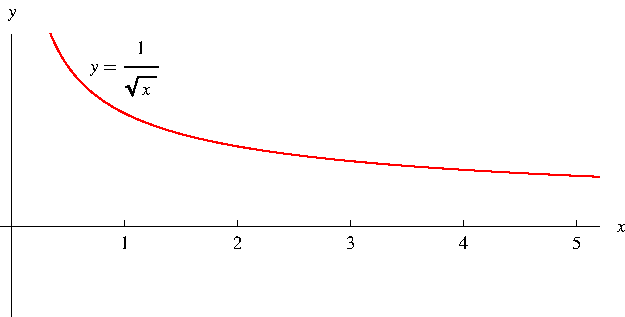
\includegraphics[width=6.5cm]{series/pictures/12-03-integral-test-belowa.pdf}%
}%
}%
\only<handout:0| 6>{%
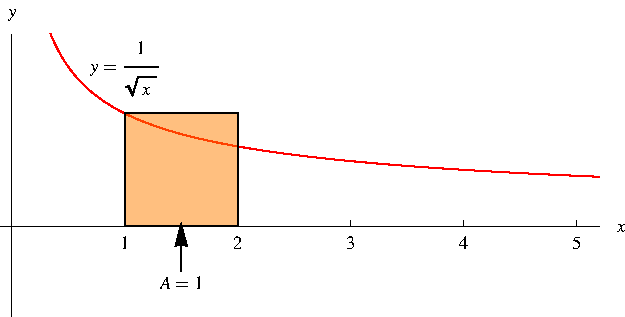
\includegraphics[width=6.5cm]{series/pictures/12-03-integral-test-belowb.pdf}%
}%
\only<handout:0| 7>{%
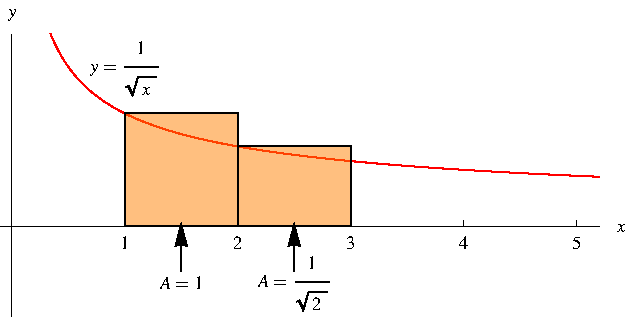
\includegraphics[width=6.5cm]{series/pictures/12-03-integral-test-belowc.pdf}%
}%
\only<handout:0| 8>{%
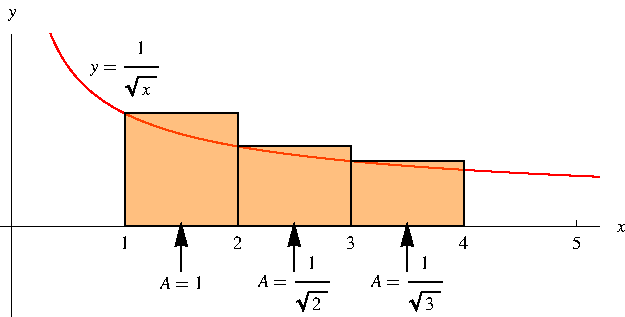
\includegraphics[width=6.5cm]{series/pictures/12-03-integral-test-belowd.pdf}%
}%
\only<handout:1| 9-10>{%
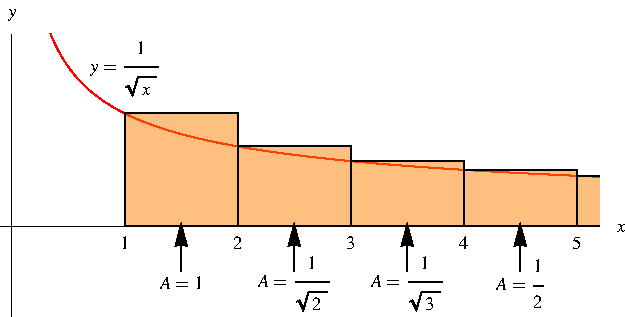
\includegraphics[width=6.5cm]{series/pictures/12-03-integral-test-belowf.pdf}%
}%
\only<handout:2| 11>{%
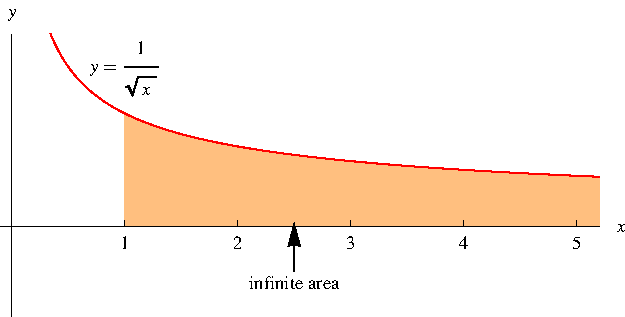
\includegraphics[width=6.5cm]{series/pictures/12-03-integral-test-belowg.pdf}%
}%
\only<handout:3| 12>{%
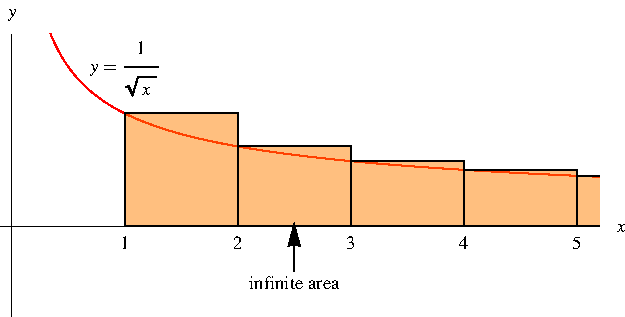
\includegraphics[width=6.5cm]{series/pictures/12-03-integral-test-belowh.pdf}%
}%
\end{center}
\column{.4\textwidth}
\uncover<2->{%
\[
\begin{array}{|r@{\ }|r|}
\hline
n & s_n = \sum_{i=1}^n \frac{1}{\sqrt{i}}\\
\hline
     5 & 3.2317 \\
    10 & 5.0210 \\
    50 & 12.7524 \\
   100 & 18.5896 \\
   500 & 43.2834 \\
  1000 & 61.8010 \\
  5000 & 139.9681 \\
\hline
\end{array}
\]
}%
\begin{itemize}
\item<6->  $\frac{1}{\sqrt{1}}$ is the area of a rectangle.
\item<7->  So is $\frac{1}{\sqrt{2}}$.
\item<handout:2-| 10-| alert@10-11>  $\int_1^\infty \frac{1}{\sqrt{x}}\diff x$ is \uncover<11->{divergent.}
\item<handout:3-| 12->  Therefore $\sum_{n=1}^\infty \frac{1}{\sqrt{n}}$ is divergent.
\end{itemize}
\end{columns}
\end{frame}
% end module integral-test-below
